% Apresentação da defesa do TCC (issue #249, critério C8 do plano de fechamento).
% Compilar com pdflatex (latexmk -pdf) a partir de text/apresentacao/.
% Regra: todo número dos slides aparece igual no texto do TCC. Cada frame anota,
% em comentário, a seção do texto de onde vem cada número e o tempo estimado.
% Tempo-alvo: até 20 min (Art. 16 do regulamento de TCC do Campus Joinville).
% Estimativa: abertura 0,3 min + 16 slides de conteúdo (de 0,9 a 1,3 min cada,
% somando 18,2 min) = 18,5 min; encerramento e reservas ficam fora do tempo.
% Revisão do orientador (#272): o piloto foi para a reserva e entrou o slide do TFT.
% As figuras recortadas vêm de ../figuras/slides/ (PNG gerado por recortes.sh), e não
% de trim + clip, que deixava a parte cortada escondida dentro do PDF.
% Os números foram escritos no formato do texto (vírgula decimal, ponto de milhar)
% e conferidos por script contra o texto das branches do fechamento do TCC.
\documentclass[aspectratio=169,10pt]{beamer}

\usepackage[T1]{fontenc}
\usepackage[brazilian]{babel}
\usepackage[sfdefault,lining]{FiraSans}
\usepackage{array}
\usepackage{booktabs}
\usepackage{graphicx}
\usepackage{appendixnumberbeamer}
\usepackage{tikz}
\usetikzlibrary{arrows.meta,positioning}

\usetheme[progressbar=frametitle,numbering=fraction,block=fill]{metropolis}
\setbeamertemplate{frame footer}{Marcelo Santos do Carmo --- Defesa de TCC}
% Destaque mais escuro que o laranja padrão do tema, para contraste no projetor.
\setbeamercolor{alerted text}{fg=mLightBrown!70!black}
% Curso e orientadores no mesmo corpo, legível na projeção.
\setbeamerfont{institute}{size=\small}

\graphicspath{{../figuras/}}

\newcommand{\hum}{\(h{+}1\)}
\newcommand{\hsete}{\(h{+}7\)}

\title{Avaliação probabilística pré-registrada do\\ \textit{Temporal Fusion Transformer}}
\subtitle{Na previsão de retornos diários da AAPL}
\author{Marcelo Santos do Carmo}
\institute{Engenharia Mecatrônica --- UFSC, Centro Tecnológico de Joinville\\[2pt]
  Orientador: Dr. Pedro Paulo de Andrade Júnior \quad Coorientador: Dr. Benjamin Grando Moreira}
\date{Defesa de Trabalho de Conclusão de Curso --- 2026}

\begin{document}

% Tempo: 0,3 min (abertura, não conta como slide de conteúdo).
\maketitle

% ---------------------------------------------------------------------------
% 1. A pergunta --- tempo: 1,0 min
% Fontes: R2 < 1% mensal e 0,4% para ações individuais (Cap. 2, Contextualização,
% e Cap. 3, Previsão de séries temporais financeiras); AAPL, h+1 e h+7
% (Cap. 2, Delimitação).
\begin{frame}{A pergunta}
  \begin{itemize}
    \item Prever o retorno de uma ação de um dia para o outro é quase impossível:
      mesmo com dados mensais, o \(R^2\) fora da amostra costuma ficar abaixo de 1\%
      (cerca de 0,4\% para ações individuais).
    \item Já o \alert{tamanho} típico do retorno (a volatilidade) é persistente:
      dias agitados tendem a vir em sequência.
    \item Por isso o objeto do trabalho não é o número previsto, e sim a
      \alert{incerteza} em torno dele.
  \end{itemize}
  \vspace{4pt}
  \begin{block}{Pergunta de pesquisa}
    Um modelo de aprendizado profundo, o \textit{Temporal Fusion Transformer} (TFT),
    descreve a distribuição do retorno de forma \alert{calibrada}? E faz isso melhor
    que modelos simples?
  \end{block}
  \vspace{2pt}
  {\small Piloto: ação da Apple (AAPL), horizontes de 1 e 7 pregões à frente (\hum{} e \hsete).}
\end{frame}

% ---------------------------------------------------------------------------
% 2. Previsão quantílica --- tempo: 1,2 min
% Fontes: sete níveis {0,02; 0,1; 0,25; 0,5; 0,75; 0,9; 0,98} (Cap. 3, Grade densa
% de quantis); faixas de 50%, 80% e 96%, mediana perto de zero, início de 2020,
% semente ilustrativa (Cap. 5, Cenários experimentais, parágrafo da Figura do fan chart).
\begin{frame}{O que é uma previsão quantílica}
  \centering
  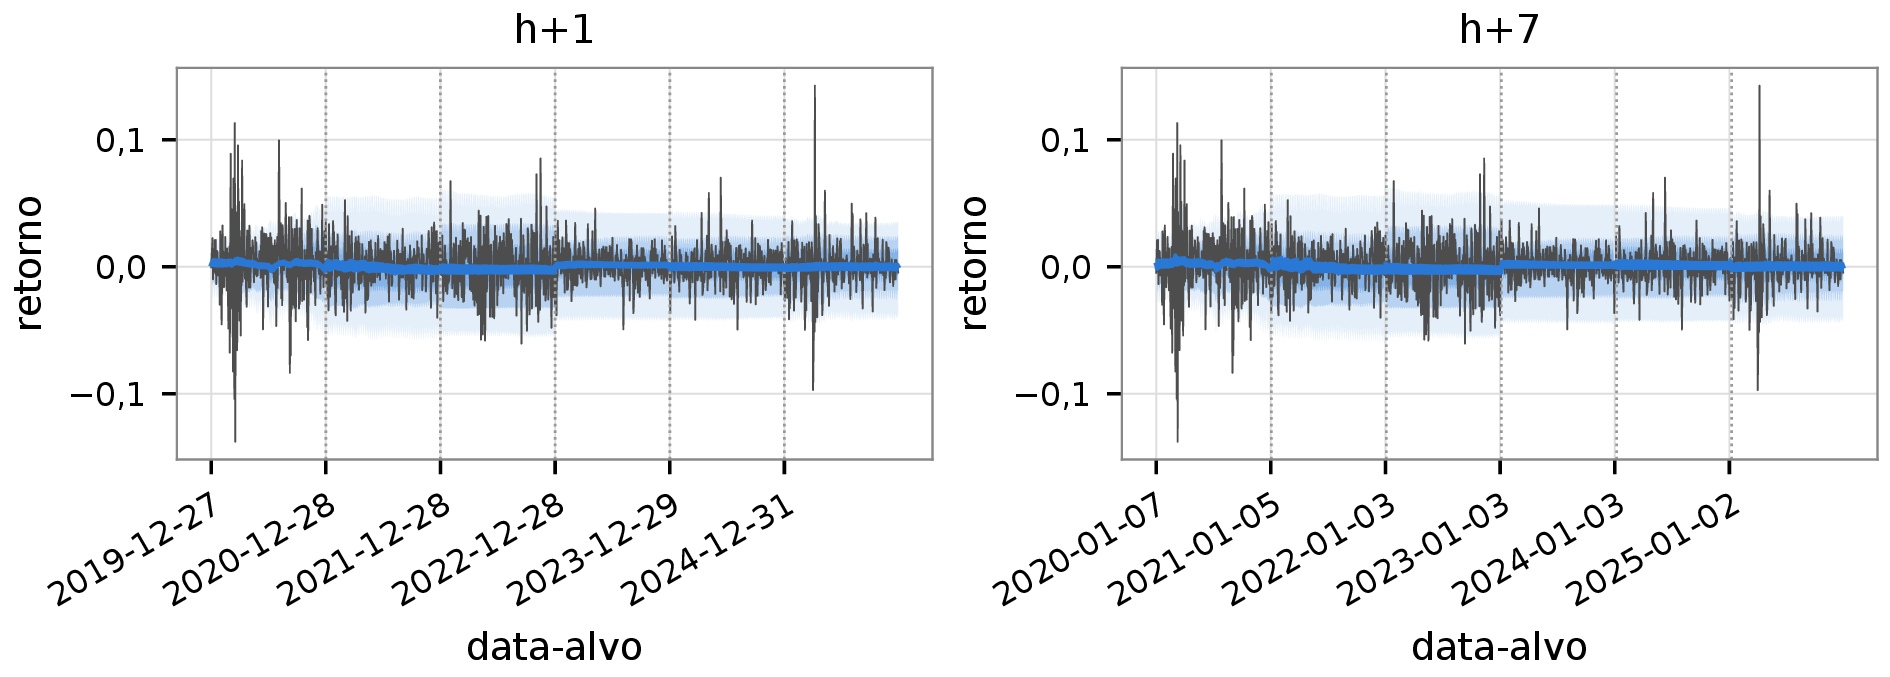
\includegraphics[width=0.9\textwidth]{slides/oos_fan_chart.png}

  \vspace{-2pt}
  \begin{columns}[T]
    \begin{column}{0.5\textwidth}
      \small
      \begin{itemize}
        \item A cada dia, o TFT emite sete quantis, de 0,02 a 0,98.
        \item As faixas formam intervalos de 50\%, 80\% e 96\%; a linha cinza é o retorno realizado.
      \end{itemize}
    \end{column}
    \begin{column}{0.5\textwidth}
      \small
      \begin{itemize}
        \item A mediana fica perto de zero: a média do retorno é quase imprevisível.
        \item Episódios como o início de 2020 escapam das faixas.
      \end{itemize}
    \end{column}
  \end{columns}
\end{frame}

% ---------------------------------------------------------------------------
% 3. Como se mede --- tempo: 1,3 min
% Fontes: pinball loss, Eq. da pinball (Cap. 3, Predição probabilística e quantílica);
% regra própria (mesma seção, Gneiting e Raftery 2007); intervalo de 80% e taxa
% nominal de 0,10 por cauda (Cap. 4, Scorecard pré-registrado; Cap. 3, Calibração);
% "não rejeitada" e poder (Cap. 3, Calibração).
\begin{frame}{Como se mede uma previsão de incerteza}
  \begin{columns}[T]
    \begin{column}{0.48\textwidth}
      \textbf{\textit{Pinball loss}} (perda quantílica)
      \[
        L_\tau(y,\hat q) = \max\bigl(\tau\,(y-\hat q),\ (\tau-1)\,(y-\hat q)\bigr)
      \]
      \centering
      \begin{tikzpicture}[x=1.5cm,y=1.3cm,font=\footnotesize]
        \draw[->] (-1.3,0) -- (1.4,0) node[below left] {\(y-\hat q\)};
        \draw[->] (0,-0.1) -- (0,1.1) node[above] {perda};
        \draw[very thick,mLightBrown] (-1.2,0.12) -- (0,0) -- (1.2,0.9);
        \node[anchor=west,align=left] at (0.75,0.3) {acima do quantil:\\ inclinação \(0{,}9\)};
        \node[anchor=south,align=center] at (-0.7,0.2) {abaixo do quantil:\\ inclinação \(0{,}1\)};
      \end{tikzpicture}

      {\small Exemplo: quantil \(\tau = 0{,}9\).}
      \par
      \raggedright
      \small Penaliza os erros de forma assimétrica. O valor esperado é mínimo
      quando o quantil informado é o verdadeiro.
    \end{column}
    \begin{column}{0.5\textwidth}
      \textbf{Calibração}
      \begin{itemize}
        \item Um intervalo de 80\% deve conter o retorno em cerca de 80\% dos dias.
        \item Em cada cauda, a taxa de violações deve ficar perto de 0,10.
        \item \textbf{Nitidez}: um intervalo estreito só é melhor com a mesma cobertura.
        \item Não rejeitar a calibração não a prova: o \alert{poder} do teste
          precisa ser declarado.
      \end{itemize}
    \end{column}
  \end{columns}
\end{frame}

% ---------------------------------------------------------------------------
% 4. Erros comuns da área --- tempo: 0,9 min
% Fontes: Cap. 2, Problema de pesquisa (erro pontual, poucos comparadores simples,
% configuração escolhida após o teste); Cap. 3, Previsão de séries temporais
% financeiras (ganhos altos = suspeita de leakage); Cap. 3, Avaliação fora da amostra
% (alinhamento temporal exato; data snooping). Sem números.
\begin{frame}{Erros comuns em previsão financeira}
  \begin{enumerate}
    \item Avaliar só o erro do valor previsto, que é cego à qualidade da incerteza.
    \item Comparar o modelo proposto com poucos modelos simples.
    \item Escolher a configuração \alert{depois} de ver o desempenho no teste
      (\textit{data snooping}): o ``melhor'' de uma busca parece significativo por acaso.
    \item Vazamento de informação futura (\textit{leakage}): ganhos altos demais são suspeitos.
    \item Calcular o erro de cada modelo sobre datas diferentes.
  \end{enumerate}
  \vspace{6pt}
  \begin{block}{Resposta deste trabalho}
    Um único candidato, comparadores declarados antes e comparação apenas
    sobre as mesmas datas: a busca é eliminada, em vez de corrigida.
  \end{block}
\end{frame}

% ---------------------------------------------------------------------------
% 6. Objetivo e hipóteses --- tempo: 1,1 min
% Fontes: Cap. 2, Objetivo geral e Hipóteses; intervalo de 80% (Cap. 4, Scorecard);
% critério de sucesso (Cap. 4, Scorecard, item Vencedor primário).
\begin{frame}{Objetivo e hipóteses}
  \textbf{Objetivo:} caracterizar a calibração de um TFT quantílico, compará-lo a uma
  hierarquia de modelos de referência e descrever a contribuição de famílias de
  indicadores, sob protocolo pré-registrado.

  \vspace{6pt}
  \begin{description}[H3]
    \item[H1] \textbf{Calibração}: a calibração do intervalo de 80\% não é rejeitada
      em ao menos um horizonte, com o poder do teste declarado. É condição para H2.
    \item[H2] \textbf{Desempenho relativo}: supera os modelos ingênuos; o interesse é
      superar ou empatar com os fortes. Não dominar é resultado válido.
    \item[H3] \textbf{Famílias}: a contribuição das quatro famílias muda entre
      \hum{} e \hsete{} (descritiva, sem leitura causal).
  \end{description}
  \vspace{4pt}
  \begin{block}{Critério de sucesso, fixado antes da execução}
    H1 não rejeitada em ao menos um horizonte, independentemente de H2.
  \end{block}
\end{frame}

% ---------------------------------------------------------------------------
% 7. Dados e protocolo --- tempo: 1,3 min
% Fontes: fontes de dados e FinBERT (Cap. 4, Dados); 55 features, 17/17/11/10
% (Cap. 4, Engenharia de features, Tabela de famílias); seis folds, 252 sessões,
% embargo de 7, h_max = 7 (Cap. 4, Protocolo experimental); dez sementes (idem);
% 27 de dezembro de 2019 a 31 de dezembro de 2025, n = 1.511 e 1.505
% (Cap. 5, Cenários experimentais).
\begin{frame}{Dados e protocolo de avaliação}
  \begin{columns}[T]
    \begin{column}{0.4\textwidth}
      \small
      \textbf{Dados diários de AAPL}
      \begin{itemize}
        \item Cotações do Yahoo Finance (ajustadas por desdobramentos), notícias e
          demonstrativos da API Alpha Vantage (sentimento por FinBERT) e o calendário
          de pregão.
        \item 55 indicadores em quatro famílias: preço (17), técnico (17),
          sentimento (11) e fundamento (10).
        \item Nenhum indicador usa dados de datas posteriores à decisão,
          verificado por teste.
      \end{itemize}
    \end{column}
    \begin{column}{0.58\textwidth}
      \centering
      \begin{tikzpicture}[x=0.52cm,y=0.5cm,font=\scriptsize]
        \foreach \r/\tr/\lab in {0/3/janela 1, 1/4.4/janela 2, 2.6/7.2/janela 6} {
          \pgfmathsetmacro{\a}{\tr}
          \pgfmathsetmacro{\b}{\a+0.3}
          \pgfmathsetmacro{\c}{\b+1.4}
          \pgfmathsetmacro{\d}{\c+0.3}
          \pgfmathsetmacro{\e}{\d+1.4}
          \pgfmathsetmacro{\f}{\e+0.3}
          \pgfmathsetmacro{\g}{\f+1.4}
          \draw[fill=mDarkTeal!25] (0,-\r) rectangle (\a,-\r-0.8);
          \draw[fill=black!60] (\a,-\r) rectangle (\b,-\r-0.8);
          \draw[fill=mDarkTeal!10] (\b,-\r) rectangle (\c,-\r-0.8);
          \draw[fill=black!60] (\c,-\r) rectangle (\d,-\r-0.8);
          \draw[fill=mLightBrown!40] (\d,-\r) rectangle (\e,-\r-0.8);
          \draw[fill=black!60] (\e,-\r) rectangle (\f,-\r-0.8);
          \draw[fill=mLightGreen!60] (\f,-\r) rectangle (\g,-\r-0.8);
          \node[left] at (0,-\r-0.4) {\lab};
        }
        \node at (2,-2.1) {\(\vdots\)};
        \draw[->] (0,-3.9) -- (12.6,-3.9) node[below left] {tempo};
        \node[anchor=north west,align=left] at (-1.5,-4.3) {
          \tikz\draw[fill=mDarkTeal!25] (0,0) rectangle (0.3,0.2); ajuste \quad
          \tikz\draw[fill=mDarkTeal!10] (0,0) rectangle (0.3,0.2); parada antecipada \quad
          \tikz\draw[fill=mLightBrown!40] (0,0) rectangle (0.3,0.2); calibração \\
          \tikz\draw[fill=mLightGreen!60] (0,0) rectangle (0.3,0.2); teste \quad
          \tikz\draw[fill=black!60] (0,0) rectangle (0.3,0.2); intervalo excluído (purga + embargo)};
      \end{tikzpicture}

      \vspace{4pt}
      \raggedright\small
      \begin{itemize}
        \item Treino que cresce a cada janela; seis blocos de teste de 252 pregões,
          de 27 de dezembro de 2019 a 31 de dezembro de 2025.
        \item TFT treinado com dez sementes em cada janela.
        \item Datas comuns a todos os modelos: \(n = 1.511\) (\hum) e \(n = 1.505\) (\hsete).
      \end{itemize}
    \end{column}
  \end{columns}
\end{frame}

% ---------------------------------------------------------------------------
% 7b. O modelo --- tempo: 1,2 min (entrou no lugar do piloto, revisão do orientador, #272)
% Fontes: Cap. 3, Temporal Fusion Transformer (estágios: VSN, LSTM no codificador e no
% decodificador, atenção multi-head interpretável, saída quantílica; entradas observadas
% até t e conhecidas até t+h; VSN do codificador sem eixo de horizonte); Cap. 4,
% Engenharia de features (55 features observadas; dia da semana e mês conhecidos);
% Cap. 4, Configuração do modelo TFT (janela de 60 sessões, 4 cabeças, decodificador de
% h_max = 7 passos, pinball sobre a grade).
\begin{frame}{O modelo: \textit{Temporal Fusion Transformer}}
  \centering
  \begin{tikzpicture}[font=\scriptsize,
      tftin/.style={draw,rounded corners,fill=black!6,align=center,text width=2.5cm,minimum height=0.95cm},
      tftblk/.style={draw,rounded corners,fill=mDarkTeal!12,align=center,text width=2.0cm,minimum height=0.95cm},
      tftout/.style={draw,rounded corners,fill=mLightGreen!35,align=center,text width=2.3cm,minimum height=2.4cm},
      arr/.style={-{Latex},thick}]
    \node[tftin] (obs) at (0,0.75) {\textbf{Observadas}\\ 55 indicadores,\\ 60 pregões até \(t\)};
    \node[tftin] (kno) at (0,-0.75) {\textbf{Conhecidas}\\ dia da semana e mês,\\ até \(t+7\)};
    \node[tftblk] (vsn1) at (3.1,0.75) {Seleção de variáveis (VSN)};
    \node[tftblk] (vsn2) at (3.1,-0.75) {Seleção de variáveis (VSN)};
    \node[tftblk] (enc) at (5.75,0.75) {LSTM\\ codificador};
    \node[tftblk] (dec) at (5.75,-0.75) {LSTM\\ decodificador, 7 passos};
    \node[tftblk,minimum height=2.4cm] (att) at (8.4,0) {Atenção\\ multi-cabeça\\ (4 cabeças)};
    \node[tftout] (q) at (11.15,0) {\textbf{7 quantis}\\ por passo\\[2pt] lidos em \(h+1\)\\ e \(h+7\)};
    \draw[arr] (obs) -- (vsn1);
    \draw[arr] (kno) -- (vsn2);
    \draw[arr] (vsn1) -- (enc);
    \draw[arr] (vsn2) -- (dec);
    \draw[arr] (enc) -- (dec) node[midway,right,font=\tiny] {estado};
    \draw[arr] (enc.east) -- (att.west |- enc.east);
    \draw[arr] (dec.east) -- (att.west |- dec.east);
    \draw[arr] (att) -- (q);
  \end{tikzpicture}

  \vspace{8pt}
  \raggedright\small
  \begin{itemize}
    \item Um único modelo para todos os horizontes, treinado com a \textit{pinball loss}
      sobre os sete quantis.
    \item Preço, indicadores, sentimento e fundamentos só entram até a decisão \(t\);
      apenas o calendário é conhecido de antemão. É isso que impede o vazamento.
    \item Os pesos da VSN dizem quanto o modelo usa cada variável, mas não mudam com o
      horizonte; por isso H3 usa permutação e ablação.
  \end{itemize}
\end{frame}

% ---------------------------------------------------------------------------
% 8. Comparadores --- tempo: 0,9 min
% Fontes: Cap. 4, Baselines (lambda = 0,94; janela de 252 sessões; LightGBM com as
% mesmas features); 55 features (Cap. 4, Engenharia de features; Cap. 5, Discussão);
% 60 tentativas (Cap. 4, Configuração do modelo TFT).
\begin{frame}{Comparadores: uma escada de dificuldade}
  \small
  \begin{tabular}{>{\raggedright\arraybackslash}p{0.17\textwidth}
                  >{\raggedright\arraybackslash}p{0.75\textwidth}}
    \toprule
    \textbf{Ingênuos} & Retorno nulo e média histórica: um único valor para todos
      os quantis (sem incerteza). \\
    \addlinespace
    \textbf{Estatísticos} & AR(1); \alert{EWMA-vol}: média exponencial dos retornos ao
      quadrado, com um único parâmetro (\(\lambda = 0{,}94\)) e quantis gaussianos;
      quantis empíricos de uma janela de 252 pregões. \\
    \addlinespace
    \textbf{Aprendizado de máquina} & \textit{Gradient boosting} quantílico (GBM),
      com os mesmos 55 indicadores do TFT. \\
    \addlinespace
    \textbf{Candidato} & TFT com os sete quantis; hiperparâmetros fixados por uma
      busca exploratória de 60 tentativas que nunca viu o teste. \\
    \bottomrule
  \end{tabular}

  \vspace{8pt}
  Todos emitem a mesma grade de quantis, nas mesmas janelas e com a mesma
  informação disponível em cada data.
\end{frame}

% ---------------------------------------------------------------------------
% 9. Regras fixadas antes de olhar --- tempo: 1,2 min
% Fontes: ordem em três tempos (Cap. 4, Protocolo experimental, último parágrafo);
% banda de Wilson de 97,5%, taxa 0,10, degeneração de no máximo 1%, desvio de
% 5 pontos percentuais (Cap. 4, Scorecard, item 2); Holm alfa = 0,05, seis
% comparações, MCS alfa = 0,10, 1.000 réplicas (Cap. 4, Métricas de avaliação);
% três revisões sem acesso a resultados (Cap. 4, Scorecard, penúltimo parágrafo).
\begin{frame}{Regras fixadas antes de olhar os resultados}
  \centering
  \begin{tikzpicture}[font=\small,node distance=0.5cm,
      box/.style={draw,rounded corners,fill=mDarkTeal!10,align=center,minimum height=0.9cm,text width=3.6cm}]
    \node[box] (a) {Modelos treinados\\ e congelados};
    \node[box,right=of a] (b) {Regras registradas,\\ com \textit{hash} e data atestada};
    \node[box,right=of b,fill=mLightGreen!30] (c) {Só então: tabelas\\ e veredito};
    \draw[-{Latex}] (a) -- (b);
    \draw[-{Latex}] (b) -- (c);
  \end{tikzpicture}

  \vspace{6pt}
  \raggedright\small
  \begin{itemize}
    \item \textbf{H1}: em cada cauda do intervalo de 80\%, a taxa nominal de 0,10 deve
      ficar dentro da banda de Wilson de 97,5\%; degeneração de no máximo 1\%;
      poder declarado contra desvios de 5 pontos percentuais.
    \item \textbf{H2}: teste de Diebold-Mariano unilateral contra os seis comparadores,
      com correção de Holm (\(\alpha = 0{,}05\)), e \textit{Model Confidence Set}
      (MCS, \(\alpha = 0{,}10\), 1.000 réplicas de \textit{bootstrap}).
    \item \textbf{``Vencedor primário''}: calibrado, supera os ingênuos e está no MCS
      (ou supera todos os fortes). Ter a menor perda não é condição.
    \item Três revisões das regras, todas antes da execução e sem acesso a resultados.
  \end{itemize}
\end{frame}

% ---------------------------------------------------------------------------
% 10. H1 --- tempo: 1,3 min
% Fontes: Cap. 5, Calibração por horizonte (H1): taxas 0,0887 / 0,0936 / 0,0882 /
% 0,0938; cobertura 0,818; poder de 0,974 a 0,987; sementes de 0,772 a 0,872 em h+1
% (Cap. 6, Limitações, na branch da #248);
% Christoffersen p de no máximo 0,003 em h+1. Figura do diagrama de confiabilidade.
\begin{frame}{H1 --- Calibração: não rejeitada nos dois horizontes}
  \begin{columns}[T]
    \begin{column}{0.5\textwidth}
      \centering
      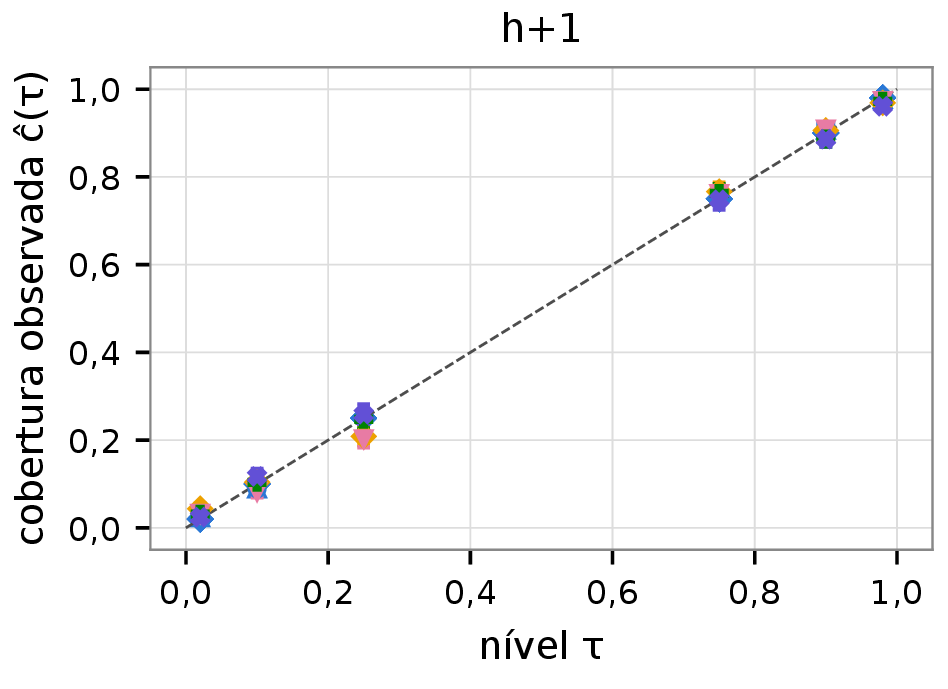
\includegraphics[height=0.55\textheight]{slides/reliability_diagram.png}

      \raggedright
      {\small Frequência observada abaixo de cada quantil, em \hum; diagonal: calibração
      perfeita. TFT em azul; comparadores, em outras cores, quase sobrepostos.
      Em \hsete, o quadro é o mesmo.}
    \end{column}
    \begin{column}{0.48\textwidth}
      \small
      \begin{tabular}{l c c}
        \toprule
        Cauda (nominal 0,10) & \hum & \hsete \\
        \midrule
        abaixo do quantil 0,10 & 0,0887 & 0,0882 \\
        acima do quantil 0,90 & 0,0936 & 0,0938 \\
        \bottomrule
      \end{tabular}

      \vspace{4pt}
      \begin{itemize}
        \item Cobertura média do intervalo de 80\%: 0,818.
        \item Poder contra desvios de 5 pontos: de 0,974 a 0,987.
        \item[\alert{!}] As violações se agrupam no tempo: a calibração é marginal, não
          condicional.
        \item[\alert{!}] Em \hum, a cobertura de uma semente isolada foi de 0,772 a 0,872.
      \end{itemize}
    \end{column}
  \end{columns}
\end{frame}

% ---------------------------------------------------------------------------
% 11. H2: perdas --- tempo: 1,1 min
% Fontes: Cap. 5, Skill relativo (H2), Tabela de pinball (x 10^-3) e o parágrafo
% seguinte: 41% a 43%; cerca de 4%; 3,3% e 1,6%.
\begin{frame}{H2 --- Perda média (\textit{pinball}, \(\times 10^{-3}\); menor é melhor)}
  \begin{columns}[T]
    \begin{column}{0.56\textwidth}
      \small
      \setlength{\tabcolsep}{4pt}
      \begin{tabular}{l l c c}
        \toprule
        & Modelo & \hum & \hsete \\
        \midrule
        Ingênuos & Retorno nulo & 6,915 & 6,924 \\
                 & Média histórica & 6,897 & 6,908 \\
        \midrule
        Estatísticos & AR(1) & 4,086 & 4,079 \\
                     & EWMA-vol & \alert{\textbf{3,920}} & \alert{\textbf{4,000}} \\
                     & Quantis empíricos & 4,037 & 4,058 \\
        \midrule
        Apr. de máquina & GBM quantílico & 3,980 & 4,026 \\
        \midrule
        Candidato & TFT & 4,050 & 4,063 \\
        \bottomrule
      \end{tabular}

      {\small TFT: média das dez sementes.}
    \end{column}
    \begin{column}{0.4\textwidth}
      \begin{itemize}
        \item Quem descreve a escala da distribuição reduz a perda dos ingênuos em
          41\% a 43\%.
        \item Entre os fortes, as diferenças são de no máximo cerca de 4\%.
        \item A menor perda é do \alert{EWMA-vol} nos dois horizontes; o TFT fica
          3,3\% (\hum) e 1,6\% (\hsete) acima.
      \end{itemize}
    \end{column}
  \end{columns}
\end{frame}

% ---------------------------------------------------------------------------
% 12. H2: veredito --- tempo: 1,2 min
% Fontes: Cap. 5, Análise estatística pareada: Holm rejeita contra os naive e contra
% nenhum forte; MCS p = 0,022 (h+1) e 0,332 (h+7); sensibilidade l = h com
% p = 0,061; veredito por horizonte; critério de sucesso.
\begin{frame}{H2 --- Veredito pela regra pré-registrada}
  \small
  \begin{itemize}
    \item Diebold-Mariano com Holm: o TFT supera os dois ingênuos nos dois horizontes
      e não supera nenhum comparador forte.
    \item \textit{Model Confidence Set}: em \hum, o TFT é eliminado (\(p = 0{,}022\));
      em \hsete, permanece (\(p = 0{,}332\)), ao lado de EWMA-vol, GBM e quantis empíricos.
  \end{itemize}
  \vspace{2pt}
  \centering
  \begin{tabular}{l c >{\raggedright\arraybackslash}p{3.3cm} >{\raggedright\arraybackslash}p{5.6cm}}
    \toprule
    Horizonte & H1 & H2 & Vencedor primário (pré-registrado) \\
    \midrule
    \hum & não rejeitada & supera só os ingênuos & não \\
    \addlinespace
    \hsete & não rejeitada & supera os ingênuos e empata com os fortes
      & sim, por \alert{empate estatístico}: a menor perda é do EWMA-vol, e o empate
        é sensível ao bloco do \textit{bootstrap} \\
    \bottomrule
  \end{tabular}

  \vspace{2pt}
  \raggedright
  \begin{alertblock}{Perto da fronteira}
    Com blocos de \(h\) pregões, o TFT sairia do MCS em \hsete{} (\(p = 0{,}061\));
    vale a especificação fixada antes da rodada.
  \end{alertblock}
\end{frame}

% ---------------------------------------------------------------------------
% 13. H3 --- tempo: 1,0 min
% Fontes: Cap. 5, Contribuição de famílias (H3), Tabela de participações s_f
% (permutação e ablação); intervalos de 98,75%; cerca de 0,5% da perda; medianas
% da VSN 0,385 / 0,253 / 0,140 / 0,127.
\begin{frame}{H3 --- Contribuição das famílias: não sustentada}
  \begin{columns}[T]
    \begin{column}{0.56\textwidth}
      \small
      \begin{tabular}{l c c c c}
        \toprule
        & \multicolumn{2}{c}{Permutação} & \multicolumn{2}{c}{Ablação} \\
        Família & \hum & \hsete & \hum & \hsete \\
        \midrule
        Técnico & 0,675 & 0,761 & 0,340 & 0,398 \\
        Preço & 0,261 & 0,199 & 0,296 & 0,301 \\
        Sentimento & 0,058 & 0,091 & 0,283 & 0,290 \\
        Fundamento & 0,006 & \(-\)0,051 & 0,081 & 0,010 \\
        \bottomrule
      \end{tabular}

      {\small Participação de cada família na importância total.}
    \end{column}
    \begin{column}{0.42\textwidth}
      \small
      \begin{itemize}
        \item Nenhum intervalo (98,75\%) da variação entre horizontes exclui o zero,
          nos dois métodos.
        \item As importâncias são pequenas: permutar a família técnica muda a perda
          em cerca de 0,5\%.
        \item A ordem é estável: a família \alert{técnica}, que reúne as medidas de
          volatilidade, vem à frente. Os pesos internos do TFT (VSN) seguem a mesma
          ordem: 0,385, 0,253, 0,140 e 0,127.
      \end{itemize}
    \end{column}
  \end{columns}
\end{frame}

% ---------------------------------------------------------------------------
% 14. Por que o EWMA-vol venceu --- tempo: 1,1 min
% Fontes: Cap. 5, Discussão, Por que o EWMA-vol teve a menor perda (GBM 3,980 contra
% 3,920; cerca de 0,5%; sementes de 3,987 a 4,117, cerca de 3%); Relação com a
% literatura (regime de uso do TFT); largura: Spearman 0,93 e 0,50 e o pico do início de
% 2020 (Seção 4.7.1, medida D4). A média das sementes está na reserva R11.
\begin{frame}{Por que o EWMA-vol teve a menor perda}
  \small
  Leitura: quase toda a informação aproveitável está no \alert{tamanho recente dos
  retornos}, que é o que a recursão do EWMA acompanha.
  \begin{enumerate}
    \item \textbf{Não é só o TFT}: o GBM, com os mesmos 55 indicadores, também perdeu
      (3,980 contra 3,920 em \hum).
    \item \textbf{As famílias acrescentam pouco}: a técnica domina e muda a perda em
      cerca de 0,5\%.
    \item \textbf{Sementes}: a perda do TFT vai de 3,987 a 4,117 entre sementes
      (cerca de 3\%), a mesma ordem da distância até o EWMA-vol.
    \item \textbf{Largura}: a do EWMA-vol acompanha a volatilidade (Spearman de 0,93);
      a do TFT, menos (0,50 em \hum). A maior desvantagem do TFT aparece no salto de
      volatilidade do início de 2020.
  \end{enumerate}
  Combinar as sementes não muda o quadro (análise exploratória, na reserva).

  \vspace{2pt}
  Hipótese não testada: o TFT foi concebido para muitas séries, com a volatilidade
  como alvo; aqui, um único ativo, com o retorno como alvo.
\end{frame}

% ---------------------------------------------------------------------------
% 15. Reprodutibilidade, delimitações e limitações --- tempo: 1,2 min
% Delimitações e limitações separadas como na Seção 5.4 (revisão do orientador, #272).
% Fontes: 1.173.254 valores, 19 tabelas, bit a bit, outro ambiente não realizado
% (Cap. 5, Cenários experimentais; Apêndice C.4); validação contra referências
% (Cap. 4, Métricas de avaliação, último parágrafo); limitações (Cap. 6, Limitações:
% um ativo; simplificações temporais; notícias 143 a 378 por ano de 2010 a 2024 e
% 3.440 em 2025); MCS sensível ao bloco e subpotência (Cap. 5, Ameaças à validade).
\begin{frame}{Reprodutibilidade, delimitações e limitações}
  \begin{columns}[T]
    \begin{column}{0.36\textwidth}
      \footnotesize
      \textbf{Reprodutibilidade}
      \begin{itemize}
        \item Veredito refeito bit a bit a partir das previsões salvas, sem novo
          treino: 1.173.254 valores de 19 tabelas, nenhuma diferença.
        \item Outro ambiente de execução: não testado.
        \item Métricas e testes conferidos contra implementações de referência,
          inclusive do R.
      \end{itemize}
    \end{column}
    \begin{column}{0.3\textwidth}
      \footnotesize
      \textbf{Delimitações} (escolhas de escopo)
      \begin{itemize}
        \item Um ativo e um período: as conclusões não se estendem a outros.
        \item Horizontes \hum{} e \hsete.
        \item Sem estratégia de negociação.
        \item Leitura das famílias preditiva, não causal.
      \end{itemize}
    \end{column}
    \begin{column}{0.32\textwidth}
      \footnotesize
      \textbf{Limitações} (do que foi medido)
      \begin{itemize}
        \item Poder baixo contra diferenças de poucos por cento entre os fortes.
        \item O empate em \hsete{} depende do bloco do \textit{bootstrap}.
        \item Simplificações temporais nas notícias e nos fundamentos, com efeito não medido.
        \item Cobertura das notícias muda em outubro de 2025: 3.440 notícias em 2025, contra
          143 a 378 por ano antes.
      \end{itemize}
    \end{column}
  \end{columns}
  \vspace{4pt}
  \centering\footnotesize Código, pré-registro e documentação de decisões:
  \texttt{github.com/MarceloSanC/financial-forecasting}\\
  Código e previsões da rodada no Zenodo: DOI \texttt{10.5281/zenodo.23843137}
\end{frame}

% ---------------------------------------------------------------------------
% 16. Conclusão e trabalhos futuros --- tempo: 1,2 min
% Fontes: Cap. 6, Síntese dos achados (poder acima de 0,97); Cap. 6, Contribuições
% empíricas (modelos de volatilidade simples como barra mínima); Cap. 6, Trabalhos
% futuros (h+30; caudas t-Student; TFT global; volatilidade assimétrica).
\begin{frame}{Conclusão e trabalhos futuros}
  \small
  \begin{itemize}
    \item \textbf{H1}: calibração não rejeitada nos dois horizontes, com poder acima
      de 0,97; ela é marginal (violações agrupadas no tempo) e vale na média das sementes.
    \item \textbf{H2}: supera os ingênuos, não os fortes; empata em \hsete; menor perda: EWMA-vol.
    \item \textbf{H3}: não sustentada; a família técnica vem à frente.
  \end{itemize}
  \begin{block}{Mensagem}
    O valor está em descrever a \alert{escala} da distribuição, não em prever a média.
    Sugere-se um modelo de volatilidade simples como barra mínima na previsão
    probabilística de retornos diários.
  \end{block}
  \textbf{Trabalhos futuros}
  \begin{itemize}
    \item TFT global, treinado sobre muitos ativos, no regime para o qual foi concebido.
    \item Comparador de volatilidade assimétrico e caudas t-Student para o EWMA.
    \item Horizontes mais longos (\(h{+}30\)) e outros ativos, com novo pré-registro.
  \end{itemize}
\end{frame}

\begin{frame}[standout]
  Obrigado!\\[6pt]
  {\normalsize Perguntas?}
\end{frame}

% ===========================================================================
% Slides de reserva (para a arguição). Não contam no tempo da apresentação.
% ===========================================================================
\appendix
% Reservas numeradas à parte (R1, R2, ...), para serem chamadas pelo número na arguição.
\setcounter{framenumber}{0}
\setbeamertemplate{frame numbering}{R\insertframenumber}

% Reserva 0 --- Estudo piloto (saiu da apresentação na revisão do orientador, #272).
% Fontes: Cap. 4, Estudo piloto e decisões de desenho (Tabela de lições do piloto):
% 685 linhas, 91,25%, três níveis, limiar de 1%, sete níveis, MCS com erro.
% O piloto não é evidência (mesma seção).
\begin{frame}{Reserva --- Estudo piloto: o que motivou o desenho}
  \small
  \begin{tabular}{>{\raggedright\arraybackslash}p{0.46\textwidth}
                  >{\raggedright\arraybackslash}p{0.46\textwidth}}
    \toprule
    \textbf{O piloto revelou} & \textbf{Decisão do desenho final} \\
    \midrule
    Previsões e valores realizados desalinhados no tempo: em \hum, nenhuma
    de 685 linhas tinha o mesmo valor realizado nas duas séries
    & Data de decisão única, contada em pregões; comparação só sobre datas comuns \\
    \addlinespace
    91,25\% das execuções avulsas com a grade colapsada em um ponto (\(p10 = p90\))
    & Teste de degeneração, com limiar de 1\% fixado antes \\
    \addlinespace
    Só três níveis de quantil
    & Grade comum de sete níveis para todos os modelos \\
    \addlinespace
    Teste estatístico feito à mão, com um erro no procedimento do MCS
    & Cada métrica e teste conferidos contra implementações de referência \\
    \bottomrule
  \end{tabular}

  \vspace{2pt}
  \alert{O piloto foi exploratório e não é evidência}: seus números descrevem falhas de
  procedimento, não desempenho.
\end{frame}

% Reserva 1 --- Fonte: Cap. 5, Análise estatística pareada, Tabela de DM.
\begin{frame}{Reserva --- Diebold-Mariano do TFT contra cada comparador}
  \small
  \centering
  \begin{tabular}{l r r c r r c}
    \toprule
    & \multicolumn{3}{c}{\hum{} (\(n = 1.511\))} & \multicolumn{3}{c}{\hsete{} (\(n = 1.505\))} \\
    Comparador & \(\bar d\) & DM & \(p_{\text{Holm}}\) & \(\bar d\) & DM & \(p_{\text{Holm}}\) \\
    \midrule
    Retorno nulo & \(-286{,}4\) & \(-34{,}74\) & \(<10^{-15}\) & \(-286{,}1\) & \(-22{,}70\) & \(<10^{-15}\) \\
    Média histórica & \(-284{,}7\) & \(-34{,}62\) & \(<10^{-15}\) & \(-284{,}4\) & \(-22{,}50\) & \(<10^{-15}\) \\
    AR(1) & \(-3{,}5\) & \(-2{,}00\) & 0,091 & \(-1{,}6\) & \(-0{,}80\) & 0,852 \\
    EWMA-vol & \(+13{,}1\) & 4,05 & 1 & \(+6{,}3\) & 1,36 & 1 \\
    Quantis empíricos & \(+1{,}3\) & 0,69 & 1 & \(+0{,}5\) & 0,21 & 1 \\
    GBM quantílico & \(+7{,}0\) & 4,08 & 1 & \(+3{,}8\) & 2,37 & 1 \\
    \bottomrule
  \end{tabular}

  \vspace{6pt}
  \raggedright
  Diferencial médio de \textit{pinball} \(\bar d = \bar L_{\text{TFT}} - \bar L_{\text{comparador}}\)
  (\(\times 10^{-5}\)); negativo favorece o TFT. Teste unilateral com a correção de pequenas amostras de
  Harvey, Leybourne e Newbold (HLN) e com Holm
  sobre os seis comparadores.
\end{frame}

% Reserva 2 --- Fonte: Cap. 5, Análise estatística pareada, Tabela do MCS
% (blocos de 65 e 64 sessões; l = sqrt(T) de 39 sessões).
\begin{frame}{Reserva --- \textit{Model Confidence Set} e sensibilidade ao bloco}
  \footnotesize
  \centering
  \begin{tabular}{l c c c c c c c c}
    \toprule
    & \multicolumn{4}{c}{\hum} & \multicolumn{4}{c}{\hsete} \\
    Modelo & Prim. & MB & \(l{=}h\) & \(l{=}\sqrt{T}\) & Prim. & MB & \(l{=}h\) & \(l{=}\sqrt{T}\) \\
    \midrule
    Retorno nulo & 0,000 & 0,000 & 0,000 & 0,000 & 0,000 & 0,000 & 0,000 & 0,000 \\
    Média histórica & 0,000 & 0,000 & 0,000 & 0,000 & 0,000 & 0,000 & 0,000 & 0,000 \\
    AR(1) & 0,004 & 0,005 & 0,000 & 0,011 & 0,053 & 0,056 & 0,004 & 0,015 \\
    EWMA-vol & \textbf{1,000} & 1,000 & 1,000 & 1,000 & \textbf{1,000} & 1,000 & 1,000 & 1,000 \\
    Quantis empíricos & \textbf{0,100} & 0,111 & 0,000 & 0,121 & \textbf{0,453} & 0,448 & 0,289 & 0,488 \\
    GBM quantílico & \textbf{0,316} & 0,293 & 0,059 & 0,274 & \textbf{0,611} & 0,613 & 0,574 & 0,637 \\
    TFT & 0,022 & 0,013 & 0,000 & 0,027 & \textbf{0,332} & 0,294 & 0,061 & 0,267 \\
    \bottomrule
  \end{tabular}

  \vspace{6pt}
  \raggedright\small
  p-valor do MCS (\(\alpha = 0{,}10\)); em negrito, os retidos na especificação primária.
  Prim.: \textit{bootstrap} estacionário com bloco pela regra pré-registrada (65 e 64
  pregões); MB: blocos móveis; \(l{=}h\) e \(l{=}\sqrt{T}\): blocos de \(h\) e de 39 pregões.
  Em \hum, o TFT fica fora em todas as quatro especificações.
\end{frame}

% Reserva 3 --- Fonte: Cap. 5, Calibração por horizonte (H1), Tabela de poder.
\begin{frame}{Reserva --- Poder do teste de calibração}
  \centering
  \begin{tabular}{l l c c}
    \toprule
    Papel & Desvio & \hum & \hsete\textsuperscript{a} \\
    \midrule
    Primário & cobertura do par \(+5\) p.p. (intervalo largo) & 0,974 & 0,976 \\
    Primário & cobertura do par \(-5\) p.p. (intervalo estreito) & 0,985 & 0,987 \\
    Primário & locação \(0{,}2\sigma\) & 0,9997 & 0,9998 \\
    Secundário & cobertura do par \(+3\) p.p. & 0,632 & 0,644 \\
    Secundário & cobertura do par \(-3\) p.p. & 0,606 & 0,629 \\
    Secundário & locação \(0{,}1\sigma\) & 0,733 & 0,746 \\
    \bottomrule
  \end{tabular}

  \vspace{6pt}
  \raggedright\small
  Probabilidade exata de o teste reprovar o TFT sob cada desvio, no \(n\) medido.
  \textsuperscript{a} Supõe violações independentes; otimista para \(h > 1\).
  Contra 3 pontos percentuais, o erro passaria despercebido em cerca de uma a cada três vezes.
\end{frame}

% Reserva 4 --- Fonte: Cap. 5, Calibração por horizonte (H1), parágrafo dos
% comparadores e Figura PICP x MPIW (GBM 0,0396 e 0,769; EWMA-vol 0,0471 e 0,827;
% TFT 0,0464 e 0,818, em h+1).
\begin{frame}{Reserva --- Cobertura contra largura dos intervalos (\hum)}
  \begin{columns}[T]
    \begin{column}{0.58\textwidth}
      \centering
      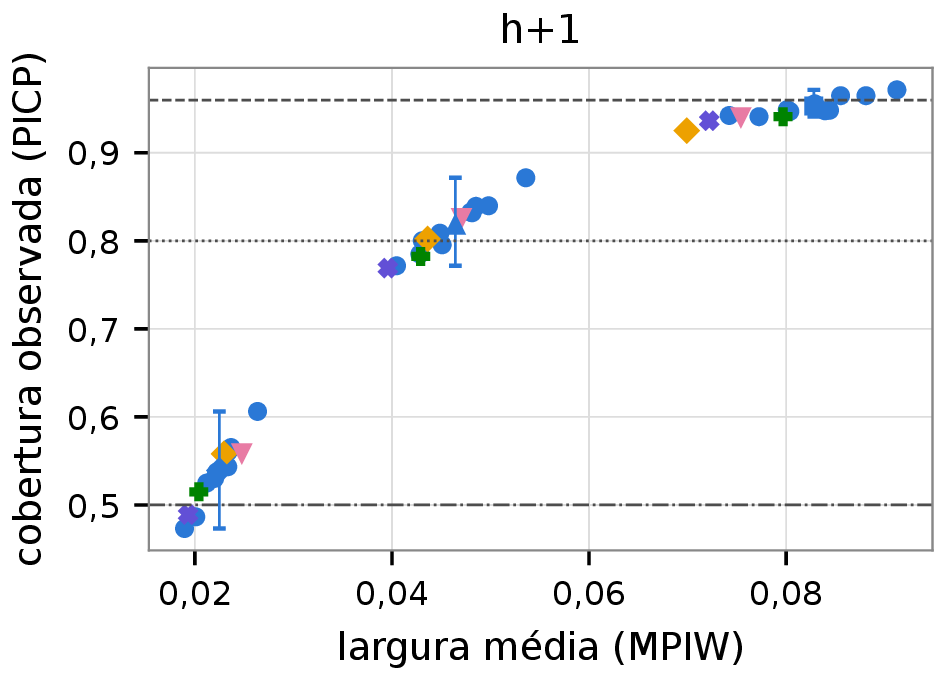
\includegraphics[height=0.68\textheight]{slides/picp_mpiw_plot.png}
    \end{column}
    \begin{column}{0.4\textwidth}
      \small
      \begin{itemize}
        \item Cada ponto: um modelo, um intervalo (50\%, 80\% ou 96\%).
          TFT em azul, GBM em roxo, EWMA-vol em rosa, AR(1) em laranja,
          quantis empíricos em verde.
        \item Linhas horizontais: as coberturas nominais.
        \item Intervalo de 80\%: GBM mais estreito (largura 0,0396) com cobertura
          de 0,769; EWMA-vol 0,0471 e 0,827; TFT 0,0464 e 0,818.
        \item O painel de \hsete{} é praticamente igual.
      \end{itemize}
    \end{column}
  \end{columns}
\end{frame}

% Reserva 5 --- Fonte: Cap. 5, Skill relativo (H2), Figura da pinball por nível e
% Tabela de pinball (mínimo e máximo entre sementes); Winkler 0,0680 / 0,0700 /
% 0,0719 / 0,0720 / 0,0728 em h+1.
\begin{frame}{Reserva --- Perda por nível de quantil e \textit{interval score}}
  \begin{columns}[T]
    \begin{column}{0.6\textwidth}
      \centering
      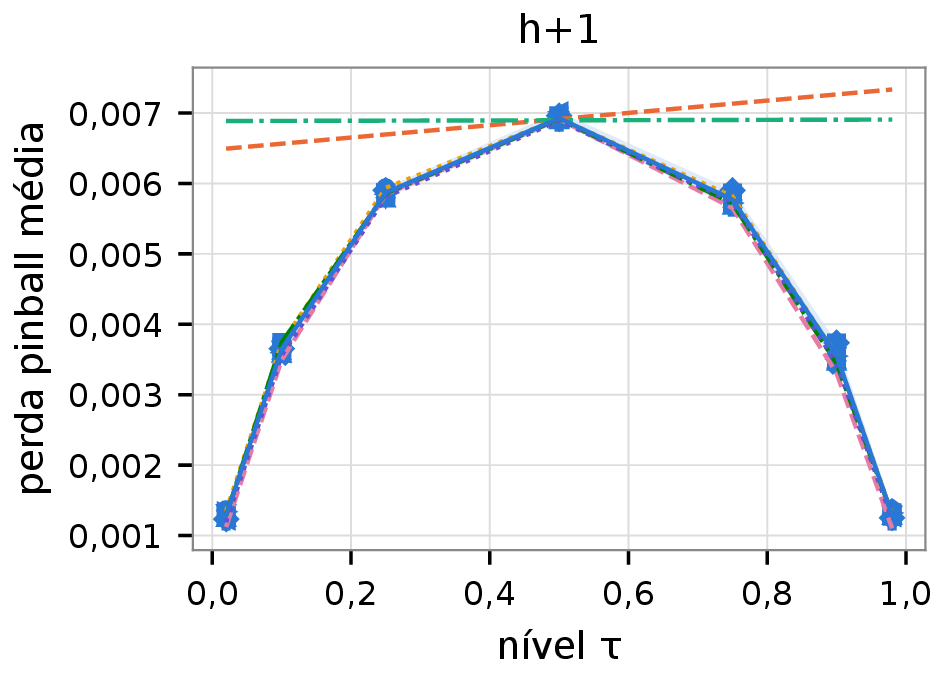
\includegraphics[height=0.58\textheight]{slides/quantile_score_plot.png}

      \raggedright
      {\small \hum. TFT em azul (as dez sementes e a média delas); ingênuos tracejados
      (retorno nulo em laranja, média histórica em verde); os demais quase se sobrepõem
      ao TFT. O painel de \hsete{} é praticamente igual.}
    \end{column}
    \begin{column}{0.38\textwidth}
      \small
      \begin{itemize}
        \item As curvas dos modelos fortes quase se sobrepõem; os ingênuos só se
          aproximam na mediana.
        \item TFT entre sementes: 3,987 a 4,117 (\hum) e 4,004 a 4,109 (\hsete).
        \item \textit{Interval score} de Winkler do intervalo de 80\% em \hum:
          EWMA-vol 0,0680; GBM 0,0700; quantis empíricos 0,0719; TFT 0,0720; AR(1) 0,0728.
      \end{itemize}
    \end{column}
  \end{columns}
\end{frame}

% Reserva 6 --- Fonte: Cap. 5, VaR descritivo, Tabela do VaR de 98%.
\begin{frame}{Reserva --- VaR descritivo de 98\% (quantil 0,02)}
  \centering\small
  \begin{tabular}{l c c c c}
    \toprule
    & \multicolumn{2}{c}{\hum} & \multicolumn{2}{c}{\hsete} \\
    Modelo & Taxa & \(p_{\text{Kupiec}}\) & Taxa & \(p_{\text{Kupiec}}\) \\
    \midrule
    AR(1) & 0,0437 & \(<0{,}001\) & 0,0445 & \(<0{,}001\) \\
    EWMA-vol & 0,0331 & \(<0{,}001\) & 0,0352 & \(<0{,}001\) \\
    Quantis empíricos & 0,0311 & 0,004 & 0,0326 & 0,001 \\
    GBM quantílico & 0,0245 & 0,229 & 0,0246 & 0,220 \\
    TFT & 0,0233 & 4 de 10 & 0,0227 & 1 de 10 \\
    \bottomrule
  \end{tabular}

  \vspace{6pt}
  \raggedright
  Nominal de 2\%. Para o TFT, média das sementes e número de sementes em que Kupiec
  rejeita. A menor perda média do EWMA-vol não se estende à cauda extrema: a forma
  gaussiana subestima caudas pesadas.
\end{frame}

% Reserva 7 --- Fonte: Cap. 5, Referência conformal (0,798; 0,800; 0,016; 0,089 para
% 0,109; NexCP 0,801 e 0,799; 96%: 0,947 contra 0,953 e 0,956).
\begin{frame}{Reserva --- Referência conformal (CQR)}
  \begin{itemize}
    \item A CQR assimétrica, calibrada no bloco de calibração de cada janela, levou a
      cobertura do intervalo de 80\% para 0,798 (\hum) e 0,800 (\hsete).
    \item Corrigiu sobretudo a cauda inferior: de 0,089 para 0,109 em \hum.
    \item A variante ponderada (NexCP) deu 0,801 e 0,799.
    \item No intervalo de 96\%, cobriu 0,947, abaixo da cobertura nativa (0,953 e 0,956).
  \end{itemize}
  \vspace{4pt}
  \begin{alertblock}{Cobertura empírica, não garantida}
    A garantia teórica da predição conformal supõe dados permutáveis, o que não vale
    em séries temporais.
  \end{alertblock}
\end{frame}

% Reserva 8 --- Fonte: Cap. 5, Perfil descritivo pontual (0,51 a 0,54; taxa-base
% 0,531; TFT 0,529 e 0,523).
\begin{frame}{Reserva --- E a acurácia direcional?}
  \begin{itemize}
    \item Fração de dias em que o sinal da mediana acerta o do retorno: entre 0,51 e 0,54.
    \item A referência certa não é 0,5, e sim a fração de dias de alta: 0,531. A média
      histórica, sempre positiva, acerta exatamente isso.
    \item O TFT fica em 0,529 (\hum) e 0,523 (\hsete), abaixo dessa taxa-base.
  \end{itemize}
  \vspace{4pt}
  \begin{block}{Leitura}
    Não há evidência de habilidade direcional, o que confirma que a média do retorno
    diário é quase imprevisível. Calculado depois do veredito, sem papel nele.
  \end{block}
\end{frame}

% Reserva 9 --- Fonte: Cap. 5, Discussão, Relação com a literatura (330 modelos;
% 1.045 séries da M3; oito métodos; nove conjuntos; 31 índices; cerca de 130 mil
% séries) e O TFT foi usado de forma pouco eficiente? (60 tentativas).
\begin{frame}{Reserva --- Relação com a literatura e uso do TFT}
  \small
  \begin{itemize}
    \item Hansen e Lunde (2005): comparando 330 modelos da família ARCH, sem evidência
      de que o GARCH(1,1) seja superado no câmbio; nos retornos da IBM, modelos com efeito
      alavancagem foram melhores. Próximo comparador natural: volatilidade assimétrica.
    \item Makridakis et al.\ (2018): em 1.045 séries mensais da M3, oito métodos
      estatísticos superaram os de aprendizado de máquina avaliados.
    \item Zeng et al.\ (2023): modelos lineares superaram \textit{Transformers} em nove
      conjuntos de previsão de longo prazo.
    \item Lim et al.\ (2021): o TFT foi avaliado com muitas séries (de dezenas a cerca
      de 130 mil); em finanças, o alvo era a volatilidade de 31 índices.
  \end{itemize}
  \begin{block}{O TFT foi mal usado?}
    Um ativo só, 60 tentativas de busca e todas as famílias sem seleção jogam contra ele,
    por escolha de escopo. Mas nada disso explica o GBM, com os mesmos indicadores,
    também ter perdido para o EWMA-vol.
  \end{block}
\end{frame}

% Reserva 10 --- Fonte: Cap. 5, Discussão, O TFT foi usado de forma pouco eficiente?
% (média das dez sementes: 1,6% e 1,4%; 3,988 e 4,008; 1,7% e 0,2% acima do EWMA-vol;
% p-valores brutos 0,98 e 0,57; dez treinos). Saiu do slide 14 para aliviá-lo.
\begin{frame}{Reserva --- Média dos quantis das sementes}
  \begin{block}{Análise exploratória, posterior ao veredito e especificada antes do cálculo}
    A média dos quantis das dez sementes reduz a perda em 1,6\% (\hum) e 1,4\% (\hsete),
    para 3,988 e 4,008. Ainda fica 1,7\% e 0,2\% acima do EWMA-vol, sem rejeição no
    Diebold-Mariano unilateral (p-valores brutos de 0,98 e 0,57), e custa dez treinos.
  \end{block}
\end{frame}

% Reserva 11 --- Fonte: Cap. 4, Scorecard (três revisões; cegamento declarado).
\begin{frame}{Reserva --- Pré-registro: o que mudou e quando}
  \begin{itemize}
    \item As regras ficam num arquivo congelado, com \textit{hash} registrado antes de
      gerar as tabelas; uma correção vira nova revisão, nunca uma edição.
    \item Três revisões, todas antes da rodada confirmatória e sem acesso a resultados,
      sem mudar nada do que julga H1 e H2:
      \begin{enumerate}
        \item regras dos perfis descritivos;
        \item regras da referência conformal;
        \item regras de H3.
      \end{enumerate}
    \item Cegamento declarado: as tabelas rodaram uma vez antes do pré-registro, num
      teste de software; nenhum valor de desempenho foi lido.
  \end{itemize}
\end{frame}

\end{document}
